\documentclass[a4paper]{article}

\usepackage{geometry}
\usepackage{booktabs}
\usepackage{minted}
\usepackage{indentfirst}
\usepackage{hyperref}
\usepackage{graphicx}

\geometry{scale=0.8}

\title{PKU-CompNet (H) Fall'22 \\ Lab Assignment (Premium): Protocol Stack \\ Report}
\author{Jiaheng Li (2000013054)}
\date{October 12, 2022}

\begin{document}
  \maketitle

  \tableofcontents

  \section{Lab 1: Link-layer}

  \subsection{Writing Task 1 (WT1)}

  The third frame in the results is:
  \begin{table}[!ht]
    \centering
    \fontsize{8pt}{8pt}
    \ttfamily
    \begin{tabular}{lllllll}
      No. & Time & Source & Destination & Protocol & Length & Info \\
      12 & 1.068164 & 0.0.0.0 & 255.255.255.255 & DHCP & 342 & DHCP Discover - Transaction ID 0x13699715
    \end{tabular}
  \end{table}

  \begin{enumerate}
    \item There are 827 frames in the filtered result. (\texttt{Dislayed: 827})
    \item The destination address of the Ethernet frame is \texttt{ff:ff:ff:ff:ff:ff}, which is the broadcast address.
    \item The 71st byte is \texttt{0x15}.
  \end{enumerate}

  \subsection{Programming Task 1 (PT1)}

  (For the convenience of later tasks, the code is reconstructed when implementing the network layer. Therefore, the description here may be different from the version submitted before in Lab 1.)

  We design the interface a bit differently from the reference in the instruction, and so do the tasks below.

  For this task, we design class \texttt{NetBase} and \texttt{Ethernet} (in \texttt{src/include/\{NetBase, Ethernet\}.h} and implementation in \texttt{src/lib/\{NetBase, Ethernet\}.c}).

  The class \texttt{NetBase} is for managing \texttt{pcap} ``devices'' and flows, while class \texttt{Ethernet} built on the former is for managing Ethernet devices (with Ethernet address...).

  Methods for the required functions are:
  \begin{minted}{cpp}
Ethernet::Device *Ethernet::addDeviceByName(const char *name);
Ethernet::Device *Ethernet::findDeviceByName(const char *name);
  \end{minted}
  while more documents are provided in the Doxygen-style comment in the header files.

  The handler (descriptor) for devices is \texttt{Ethernet::Device *}.

  The method finds the device by its name through \texttt{pcap\_findalldevs()} and gets its Ethernet address.
  Then it opens the \texttt{pcap} flow and creates the \texttt{Device} object for management.

  \subsection{Programming Task 2 (PT2)}

  The class \texttt{Ethernet} also supports sending and receiving Ethernet frames.

  Methods for the required functions are:
  \begin{minted}{cpp}
int Ethernet::send(const void *data, size_t dataLen, Addr dst, uint16_t etherType,
                   Device *dev);

using Ethernet::RecvHandler = std::function<int(const void *data, size_t dataLen,
                                                const Ethernet::RecvInfo &info)>;
void Ethernet::addOnRecv(RecvHandler handler, uint16_t etherType);
  \end{minted}

  The \texttt{sendFrame()} method simply adds the Ethernet header and send it through \texttt{pcap\_sendpacket()}.

  The \texttt{addRecvCallback()} method simply adds the callback to a list.

  To receive packets, we should call \texttt{NetBase::setup()}, \texttt{Ethernet::setup()}, and finally \texttt{NetBase::loop()}.
  \texttt{NetBase::loop()} will loop forever (if not interrupted), checking for each \texttt{pcap} devices for new receiving frames using the ``nonblocking mode'' and \texttt{pcap\_dispatch()}, and then invokes the callback from \texttt{Ethernet} (or other registered) for each frame.
  It also provides an interface for callback in each loop iteration, allowing users to handle their work.

  All the routines in the network stack library run on a single thread (and are required to do so).
  For application, they may create a separate thread for the network stack library, and work on another user thread, using something like a ``task dispatcher'' to synchronize with the loop callbacks.

  We implemented a CLI program (in \texttt{src/tools/cli/}, and will be built to \texttt{build/tools/cli}), allowing users to interactively test the library.
  It uses a task dispatcher (in \texttt{src/include/LoopDispatcher.h}) to send tasks about the network stack to the network thread, and uses mutexes to wait for completion in the user thread.

  The CLI program uses the GNU Readline Library (\texttt{libreadline-dev}) (only) for easier interaction.

  \subsection{Checkpoint 1 (CP1)}

  The typescript record is at \texttt{checkpoints/CP1/\{typescript, timing.log\}}.

  In the script, several calls to \texttt{add-device} and \texttt{find-device} in a row shows that they can correctly add (only) the valid Ethernet devices on the host, get their Ethernet addresses, and correctly find the added devices.

  \subsection{Checkpoint 2 (CP2)}

  The typescript record is at \texttt{checkpoints/CP2/\{typescript, timing.log\}}.

  We implemented the \texttt{eth-test} command in the CLI, which exchanges frames through all configured devices.
  It sends the first control message using the broadcast address and gets the real destination address through the response.
  Then the hosts exchange data simultaneously (using threads and the dispatcher), and finally print the sent and received checksum.

  In the script, the \texttt{eth\_test} tool above is simultaneously run on each of the 5 hosts in the example network provided in \texttt{vnetUtils}, using all of the 8 devices and 4 links among them.
  After the run, we can see that the sending and receiving checksum of each link matches, which shows the (basic) correctness of our sending and receiving implementation.

  \section{Lab 2: Network-layer}

  \subsection{Writing Task 2 (WT2)}

  \begin{enumerate}
    \item The ``Target MAC address'' field (bytes 32-37, indexed from 0) in the ARP Reply is the same as the Sender MAC address in the ARP Request.
    \item There are 6 packets meeting the requirement. We can see this by filtering \texttt{ip.flags.df == 0} and checking the ``Displayed'' status.
    \item The header length of IPv4 is 20 bytes, while for IPv6 it is 40 bytes.
  \end{enumerate}

  \subsection{Programming Task 3 (PT3)}

  We designed the class \texttt{IP} for handling basic IPv4 operations.

  Methods for the required functions are:
  \begin{minted}{cpp}
int IP::send(const void *data, size_t dataLen, Addr src, Addr dst,
             uint8_t protocol, SendOptions options);

using IP::RecvHandler = std::function<int(const void *data, size_t dataLen,
                                          const IP::RecvInfo &info)>;
void IP::addOnRecv(RecvHandler handler, uint8_t protocol,
                   bool promiscuous = false);
  \end{minted}

  It just works like the sending/receiving methods in the Ethernet layer, which simply adds the header and sends it to the layer below, or adds the callback to a list.

  The class \texttt{IP} has registered a callback in \texttt{Ethernet}, to receive Ethernet frames of type IP.
  It then analyzes the header and distributes the received packets to its own callbacks.

  For forwarding, we also implemented a class \texttt{IPForward} as a user to the \texttt{IP}.
  It registered a callback in \texttt{IP} and then use \texttt{IP} sending methods to forward the received packets out.

  For routing, we first have the static routing in class \texttt{LpmRouting} (which derivates from the abstract \texttt{IP::Routing}), which implements the Longest Prefix Match in a static table manually added by the user.
  It then supports the \texttt{IP} class to send packets out. (ARP protocol also participates in this process, see the writing task below).

  It has the interface:
  \begin{minted}{cpp}
int LpmRouting::query(const Addr &dst, HopInfo &res) override;
int LpmRouting::setEntry(const Entry &entry);
  \end{minted}
  The \texttt{waitingCallback} is for handling the waiting for ARP replies, as will be described in the tasks below.

  We also have a dynamic routing algorithm, the (non-standard) \texttt{RIP} with similar interfaces, and cooperates with other ``routers'' in the network, which will also be described in the tasks below.

  \subsection{Writing Task 3 (WT3)}

  To send an IP packet, we first need the routing algorithm (or routing table) to find the IP (gateway) address of the next hop, or find out that they are directly connected.

  Then, we get the IP address of the exact next hop.
  We can check the ARP table, or send an ARP Request (on misses) to get the MAC address of the next hop.

  However, sending the ARP Request brings the problem of the non-immediate sending of our packets.
  It is impossible to wait for the ARP Response in our network thread.
  Therefore, the sending method will return an error.
  For convenience, we also implement the automatic resend (with callback) option in \texttt{IP::SendOptions} and maybe in the upper layers, by registering a resending callback in the ARP Response receiving procedure.
  In the user thread, we can also use a mutex to wait for the completion of resending.
  In this way, this problem will not bring too much complexity to coding.

  We implement the ARP sending method and responder in the class \texttt{ARP}, which may be called by the routing classes to find exactly the MAC address of the next hop.
  \begin{minted}{cpp}
int ARP::query(L3::Addr target, L2::Addr &res);
int ARP::sendRequest(L3::Addr target);
void ARP::handleRecv(const void *buf, size_t len, const L2::RecvInfo &info);

using ARP::WaitHandler = std::function<void(bool succ)>;
void ARP::addWait(L3::Addr addr, WaitHandler handler, Timer::Duration timeout = 60s);
  \end{minted}

  \subsection{Writing Task 4 (WT4)}

  We use a distance vector algorithm similar to the Routing Information Protocol (RIP). It is implemented in the class \texttt{RIP}.

  For the routing in the same subnet, we assume (in default) that they can reach each other directedly (so we only need the ARP protocol to get its MAC address), so their gateway is set to \texttt{0.0.0.0}, and metrics are set to $0$.

  Then, for each subnet, we maintain an element in the distance vector about the minimum hops to reach that subnet.
  We may also need the next hop (gateway) to reach that subnet, as well as the expiring time for updating.

  Every 30 seconds (or other custom value), each router will broadcast its distance vector to its neighbors.
  And when a router receives a RIP ``Response'', it could update its own distance vector (and updates the next hop or other information at the same time):
  $$d_i \gets \min\{d_i, \mathit{recv}_i + 1\},$$
  while we use $16$ as infinity, every distance larger than $16$ will be ignored.

  In this way, with sufficient broadcasts, we can find the path of minimal number of hops to each subnet, and then the router in the subnet will directly forward it to the host.

  To handle the changes or failures, every entry will be expired in 180 seconds (by setting its metric to $16$), and then after 120 seconds, it will be deleted from the routing table.

  Also, when a host adds to a network, it will immediately send an RIP Request, to get the information from its neighbors, to set up quickly.

  To optimize the handling of changes, we also use triggered update, which means to broadcast the RIP response as soon as any metric changes in our vector.
  Also, if we receive the new distance from our best choice before, we will take it even if it is worse than our metric before. These methods can significantly improve performance in changes or failures, especially for the problem of ``counting to infinity'' slowly.

  The RIP protocol runs on the UDP port 520 (with UDP broadcasts), therefore we also implement the class \texttt{UDP} over our \texttt{IP}.

  \subsection{Testing}

  We have tested the implementation in several ways. For example, in the example virtual network, our network stack could correctly forwards ICMP messages from the Linux \texttt{ping} on hosts connected through several ``routers''.

  We also implemented a simple tool in the CLI like \texttt{nc -u}, just called \texttt{nc-u} in our CLI, to send messages through UDP. They cooperates correctly in the network.

  To work with the Linux \texttt{nc} program, we need to disable the TCP/UDP checksum overload in the system using:
  \begin{minted}{bash}
ethtool -K <device> rx off tx off sg off tso off
  \end{minted}
  After that, our program can correctly cooperate with the Linux \texttt{nc}.
  It can also correctly forward the traffic of \texttt{iperf}.

  For testing, we also implemented (part of) the ICMP protocol (sender and automatic responder), and our \texttt{ping} and \texttt{traceroute} command in the CLI.
  They cooperate correctly with each other, or with the Linux system responders/programs (if we do not disable the kernel network stack).

  \subsection{Checkpoint 3 (CP3)}

  The typescript record is at \texttt{checkpoints/CP3/\{typescript, timing.log\}}.

  The hex dump of the packet is:
  \begin{minted}{text}
08:36:33.694000 IP localhost > localhost: ICMP echo request, id 45298, seq 1, length 32
        0x0000:  9af1 db8d 59ba 4247 83b2 2ecc 0800 4500  ....Y.BG......E.
        0x0010:  0034 0000 4000 4001 21ff 0a64 0101 0a64  .4..@.@.!..d...d
        0x0020:  0302 0800 3b3f b0f2 0001 4c61 622d 4e65  ....;?....Lab-Ne
        0x0030:  7453 7461 636b 2050 696e 6720 5465 7374  tStack.Ping.Test
        0x0040:  0a00                                     ..
  \end{minted}

  The first 14 bytes are the Ethernet header:
  \begin{itemize}
    \item \texttt{0x9af1db8d59ba}: Destination Address (6)
    \item \texttt{0x424783b22ecc} Source Address (6);
    \item \texttt{0x0800}: EtherType (2), IPv4.
  \end{itemize}
  The next 20 bytes are the IPv4 header, each:
  \begin{itemize}
    \item \texttt{0x4}: IPv4 version, \texttt{0x5}: IHL;
    \item \texttt{0x00}: Type of Service.
    \item \texttt{0x0034}: Total Length.
    \item \texttt{0x0000}: Identification for fragments.
    \item \texttt{0b010}: Flags (\texttt{1} for Don't fragment). The other part of \texttt{0x4000} for fragment offset.
    \item \texttt{0x40}: Time to Live.
    \item \texttt{0x01}: Protocol (ICMP).
    \item \texttt{0x21ff}: Header checksum.
    \item \texttt{0x0a640101}: Source Address: \texttt{10.100.1.1};
    \item \texttt{0x0a640302}: Destination Address: \texttt{10.100.3.2};
  \end{itemize}
  The other 32 bytes are the ICMP Echo (ping) Request message with data.
  \begin{itemize}
    \item \texttt{0x8}: Opcode, ICMP Echo (ping) Request.
    \item \texttt{0x0}: Code, 0 for Echo Request.
    \item \texttt{0x3b3f}: Checksum
    \item \texttt{0xb0f2}: Identifier
    \item \texttt{0x0001}: Sequence number
    \item Others are the data: \texttt{"Lab-NetStack Ping Test"}...
  \end{itemize}

  \subsection{Checkpoint 4 (CP4)}

  The typescript record is at \texttt{checkpoints/CP4/\{typescript, timing.log\}}.

  We use the automatic configuring command in our CLI, which configures the IP, netmask as the \texttt{vnetUtils} set to the Linux system, and turn on the RIP dynamic routing as we pass the \texttt{-r} option.

  We can see that, when we run the routing on all the hosts, ns1 can successfully ping to ns4.

  After we kill the process in ns2, n1 cannot reach other hosts anymore. We can see that the routing table finally (after expiring and cleaning time) contains only its own subnet, as ns2 is on the only way from ns1 to other hosts.

  After we run the routing in ns2 again, ns1 can reach ns4 again.

  \subsection{Checkpoint 5 (CP5)}

  The typescript record is at \texttt{checkpoints/CP5/\{typescript, timing.log\}}.

  The output file is at \texttt{checkpoints/CP5/outs/ns*.out}.

  We use the \texttt{traceroute} command in our CLI to measure the distance, we can see that it's exactly one TTL decrease for a hop.

  The distances before disconnecting ns5 are in the left table (the number on row $x$, column $y$ indicates the distance from $x$ to $y$), while the distances after disconnecting are in the right one.

  \begin{center}
    \begin{tabular}{c|cccccc}
      \toprule
      & ns1 & ns2 & ns3 & ns4 & ns5 & ns6 \\
      \midrule
      ns1 & - & $1$ & $2$ & $3$ & $2$ & $3$ \\
      ns2 & $1$ & - & $1$ & $2$ & $1$ & $2$ \\
      ns3 & $2$ & $1$ & - & $1$ & $2$ & $1$ \\
      ns4 & $3$ & $2$ & $1$ & - & $3$ & $2$ \\
      ns5 & $2$ & $1$ & $2$ & $3$ & - & $1$ \\
      ns6 & $3$ & $2$ & $1$ & $2$ & $1$ & - \\
      \bottomrule
    \end{tabular}
    \hspace{2em}
    \begin{tabular}{c|cccccc}
      \toprule
      & ns1 & ns2 & ns3 & ns4 & ns6 \\
      \midrule
      ns1 & - & $1$ & $2$ & $3$ & $3$ \\
      ns2 & $1$ & - & $1$ & $2$ & $2$ \\
      ns3 & $2$ & $1$ & - & $1$ & $1$ \\
      ns4 & $3$ & $2$ & $1$ & - & $2$ \\
      ns6 & $3$ & $2$ & $1$ & $2$ & - \\
      \bottomrule
    \end{tabular}
  \end{center}

  We can see that the minimum distances do not change even if we disconnect ns5, and our routing implementation can find still the shorted path after disconnection.

  \subsection{Checkpoint 6 (CP6)}

  The typescript record is at \texttt{checkpoints/CP6/\{typescript, timing.log\}}.

  If we use the topology as CP5 (configuration file at \texttt{checkpoints/CP6/vnet.txt} showing the IPs), we could manually config the routing table of ns5 as follows:
  \begin{minted}{text}
route-add 10.100.3.1 255.255.255.255 veth2-3 10.100.2.2
route-add 10.100.3.0 255.255.255.0 veth2-5 10.100.4.2
route-add 10.100.0.0 255.255.0.0 veth2-3 10.100.2.2
route-add 10.100.1.0 255.255.255.0 veth2-1 10.100.1.1
  \end{minted}

  Then we run other hosts as routers automatically, and try some \texttt{traceroute}, we will find:
  \begin{minted}{text}
ns2 - 10.100.3.1 (ns3)
ns2 - 10.100.4.2 (ns5) - 10.100.5.2 (ns6) - 10.100.6.1 (ns3) - 10.100.3.2 (ns4)
ns2 - 10.100.2.2 (ns3) - 10.100.6.2 (ns6) - 10.100.4.2 (ns5)
ns2 - 10.100.2.2 (ns3) - 10.100.5.2 (ns6)
ns2 - 10.100.2.2 (ns3) - 10.100.6.2 (ns6)
  \end{minted}
  It just behaves like we apply the "longest prefix matching" rule on the destination.


  \section{Lab 3: Transport-layer}

  \subsection{Writing Task 5 (WT5)}

  \begin{enumerate}
    \item In ``Statistics'' -- ``Conversations'' -- ``TCP'', we can see that we have 2 sessions:
    \begin{center}
      \begin{tabular}{c|ccc}
        \toprule
        Session & A & B & \# Segments \\
        \midrule
        1 & \texttt{10.0.0.74:43120} & \texttt{115.27.207.221:80} & $12$ \\
        2 & \texttt{10.0.0.74:43122} & \texttt{115.27.207.221:80} & $1652$ \\
        \bottomrule
      \end{tabular}
    \end{center}

    \item The list is shown in the table above.
    \item The receiving window size is
      $$85 \times 2^9 = 43520,$$
      where $85$ is the \texttt{TCP.WND} field of packet \#86, and $9$ is from the last option in the \texttt{SYN} segment (packet \#72):
      \begin{center}
        \texttt{03 03 09 | TCP Option - Kind: Window Scale (3), Length: 3, Shift Count: 9.}
      \end{center}
  \end{enumerate}

  \subsection{Programming Task 4 (PT4)}

  The required POSIX functions are implemented in \texttt{src/lib/socket.cpp}.

  To implement TCP, we defined:
  \begin{minted}{cpp}
class TCP;
class TCP::Desc;
class TCP::Listener : public TCP::Desc;
class TCP::Connection : public TCP::Desc;
  \end{minted}
  while \texttt{TCP} provides the interface from the lower (\texttt{IP}...) layers;
  \texttt{TCP::Desc} represents a ``file descriptor'';
  \texttt{TCP::Listener} represents a passive listener (a server);
  and \texttt{TCP::Connection} represents a normal connection (with a state and TCB) in which most of the TCP logic is implemented.

  We have (some of) their interfaces:
  \begin{minted}{cpp}
TCP::Desc *TCP::create();
TCP::Listener *TCP::listen(Desc *desc);
TCP::Connection *TCP::connect(Desc *desc, Sock dst);

virtual int TCP::Desc::bind(Sock sock);
virtual int TCP::Desc::awaitClose();

TCP::Connection *TCP::Listener::awaitAccept();

ssize_t TCP::Connection::send(const void *data, size_t dataLen);
ssize_t TCP::Connection::asyncSend(const void *data, size_t dataLen);
ssize_t TCP::Connection::asyncSendAll(const void *data, size_t dataLen);
ssize_t TCP::Connection::recv(void *data, size_t maxLen);
ssize_t TCP::Connection::awaitRecv(void *data, size_t maxLen);
  \end{minted}
  For safety, methods beginning with \texttt{async} or \texttt{await} should be called in threads other of the net-stack thread, while others must be called in the thread of net-stack itself.

  The event processing is implemented as the RFC in the methods above, or the receiving handlers:
  \begin{minted}{cpp}
void TCP::handleRecv(const void *seg, size_t tcpLen, const L3::RecvInfo &info);
void TCP::Listener::handleRecv(const void *seg, size_t tcpLen, const L3::RecvInfo &info);
void TCP::Connection::handleRecv(const void *seg, size_t tcpLen, const L3::RecvInfo &info);
  \end{minted}

  Implementation details can be seen in \texttt{src/lib/TCP.cpp}.

  For sending, we copy the sent data for each segment and set a timer to retransmit (using the Selective-Repeat method).
  When the sending window is full, the \texttt{asyncSend} method will be blocked until available.

  For receiving, we buffer the data for each \texttt{Connection}.
  When there is no pending data to be received, the \texttt{awaitRecv} method will be blocked until available.

  The \texttt{awaitClose} (in normal cases) will send the \texttt{FIN}, and block until the remote side closes or acknowledges the \texttt{FIN} (just as described in RFC).
  This can also make both sides close normally when the process exit (unlike the kernel stack, we cannot response anymore after the process terminates).

  To protect thread safety, we still use the \texttt{Dispatcher} for communication between threads, and the \texttt{Timer} in a single thread (by simple polling, together with receiving) to serve the TCP (and the RIP before).

  For early testing, before the POSIX interface, we also implemented a simple echo tool in our CLI, and it can cooperate correctly with Linux programs (e.g. \texttt{nc}).

  \subsection{Checkpoint 7 (CP7)}

  The typescript record is at \texttt{checkpoints/CP7/\{typescript, timing.log\}}.

  We run the \texttt{perf\_server} and \texttt{perf\_client} (both using wrapped socket functions in our implementation) on \texttt{ns1} and \texttt{ns2} of the example VNet, respectively.

  We captured the first TCP packet from \texttt{perf\_server}.

  The hex dump of the packet is:
  \begin{minted}{text}
00:57:27.448784 IP bogon.10086 > localhost.57163: Flags [S.], seq 2482714633, ack 2482711534,
win 65535, length 0
        0x0000:  02cd 0174 60da 6af4 663c 6025 0800 4500  ...t`.j.f<`%..E.
        0x0010:  0028 0000 4000 3c06 2806 0a64 0101 0a64  .(..@.<.(..d...d
        0x0020:  0102 2766 df4b 93fb 3809 93fb 2bee 5012  ..'f.K..8...+.P.
        0x0030:  ffff 0668 0000                           ...h..
  \end{minted}

  The TCP header contains 20 bytes (from byte \#0x22)
  \begin{itemize}
    \item \texttt{0x2766}: Source Port -- $10086$.
    \item \texttt{0xdf4b}: Destination Port -- $57163$.
    \item \texttt{0x93fb3809}: Sequence Number.
    \item \texttt{0x93fb2bee}: Acknowledgement Number.
    \item \texttt{0x50}: \begin{itemize}
      \item \texttt{0b0101}: Header Length -- $5$ ($20$ bytes)
      \item the other 4 bits \texttt{0b00} are reserved.
    \end{itemize}
    \item \texttt{0x12}: Flags -- \texttt{SYN}, \texttt{ACK};
    \item \texttt{0xffff}: Window -- $65535$;
    \item \texttt{0x0668}: Checksum;
    \item \texttt{0x0000}: Urgent Pointer.
  \end{itemize}

  \subsection{Checkpoint 8 (CP8)}

  The typescript record is at \texttt{checkpoints/CP8/\{typescript, timing.log\}}.

  We run the \texttt{echo\_server} and \texttt{echo\_client\_check} (added correctness checking to \texttt{echo\_client}), both using wrapped socket functions in our implementation, on \texttt{ns1} and \texttt{ns2} of the example VNet, respectively.

  We set the the following \texttt{netem} arguments to the both side (in \texttt{utils/netem.sh}):
  \begin{minted}{bash}
tc qdisc add dev $1 root netem delay 30ms 10ms loss random 10% corrupt 10% \
    duplicate 10% reorder 10%
  \end{minted}

  We can see from the result, that despite the loss and corruption of the network, the application is correct.

  (Part of) the trace is shown as Figure~\ref{fig:CP8} (the trace is at \texttt{checkpoints/CP8/capture.pcap}):

  \begin{figure}
    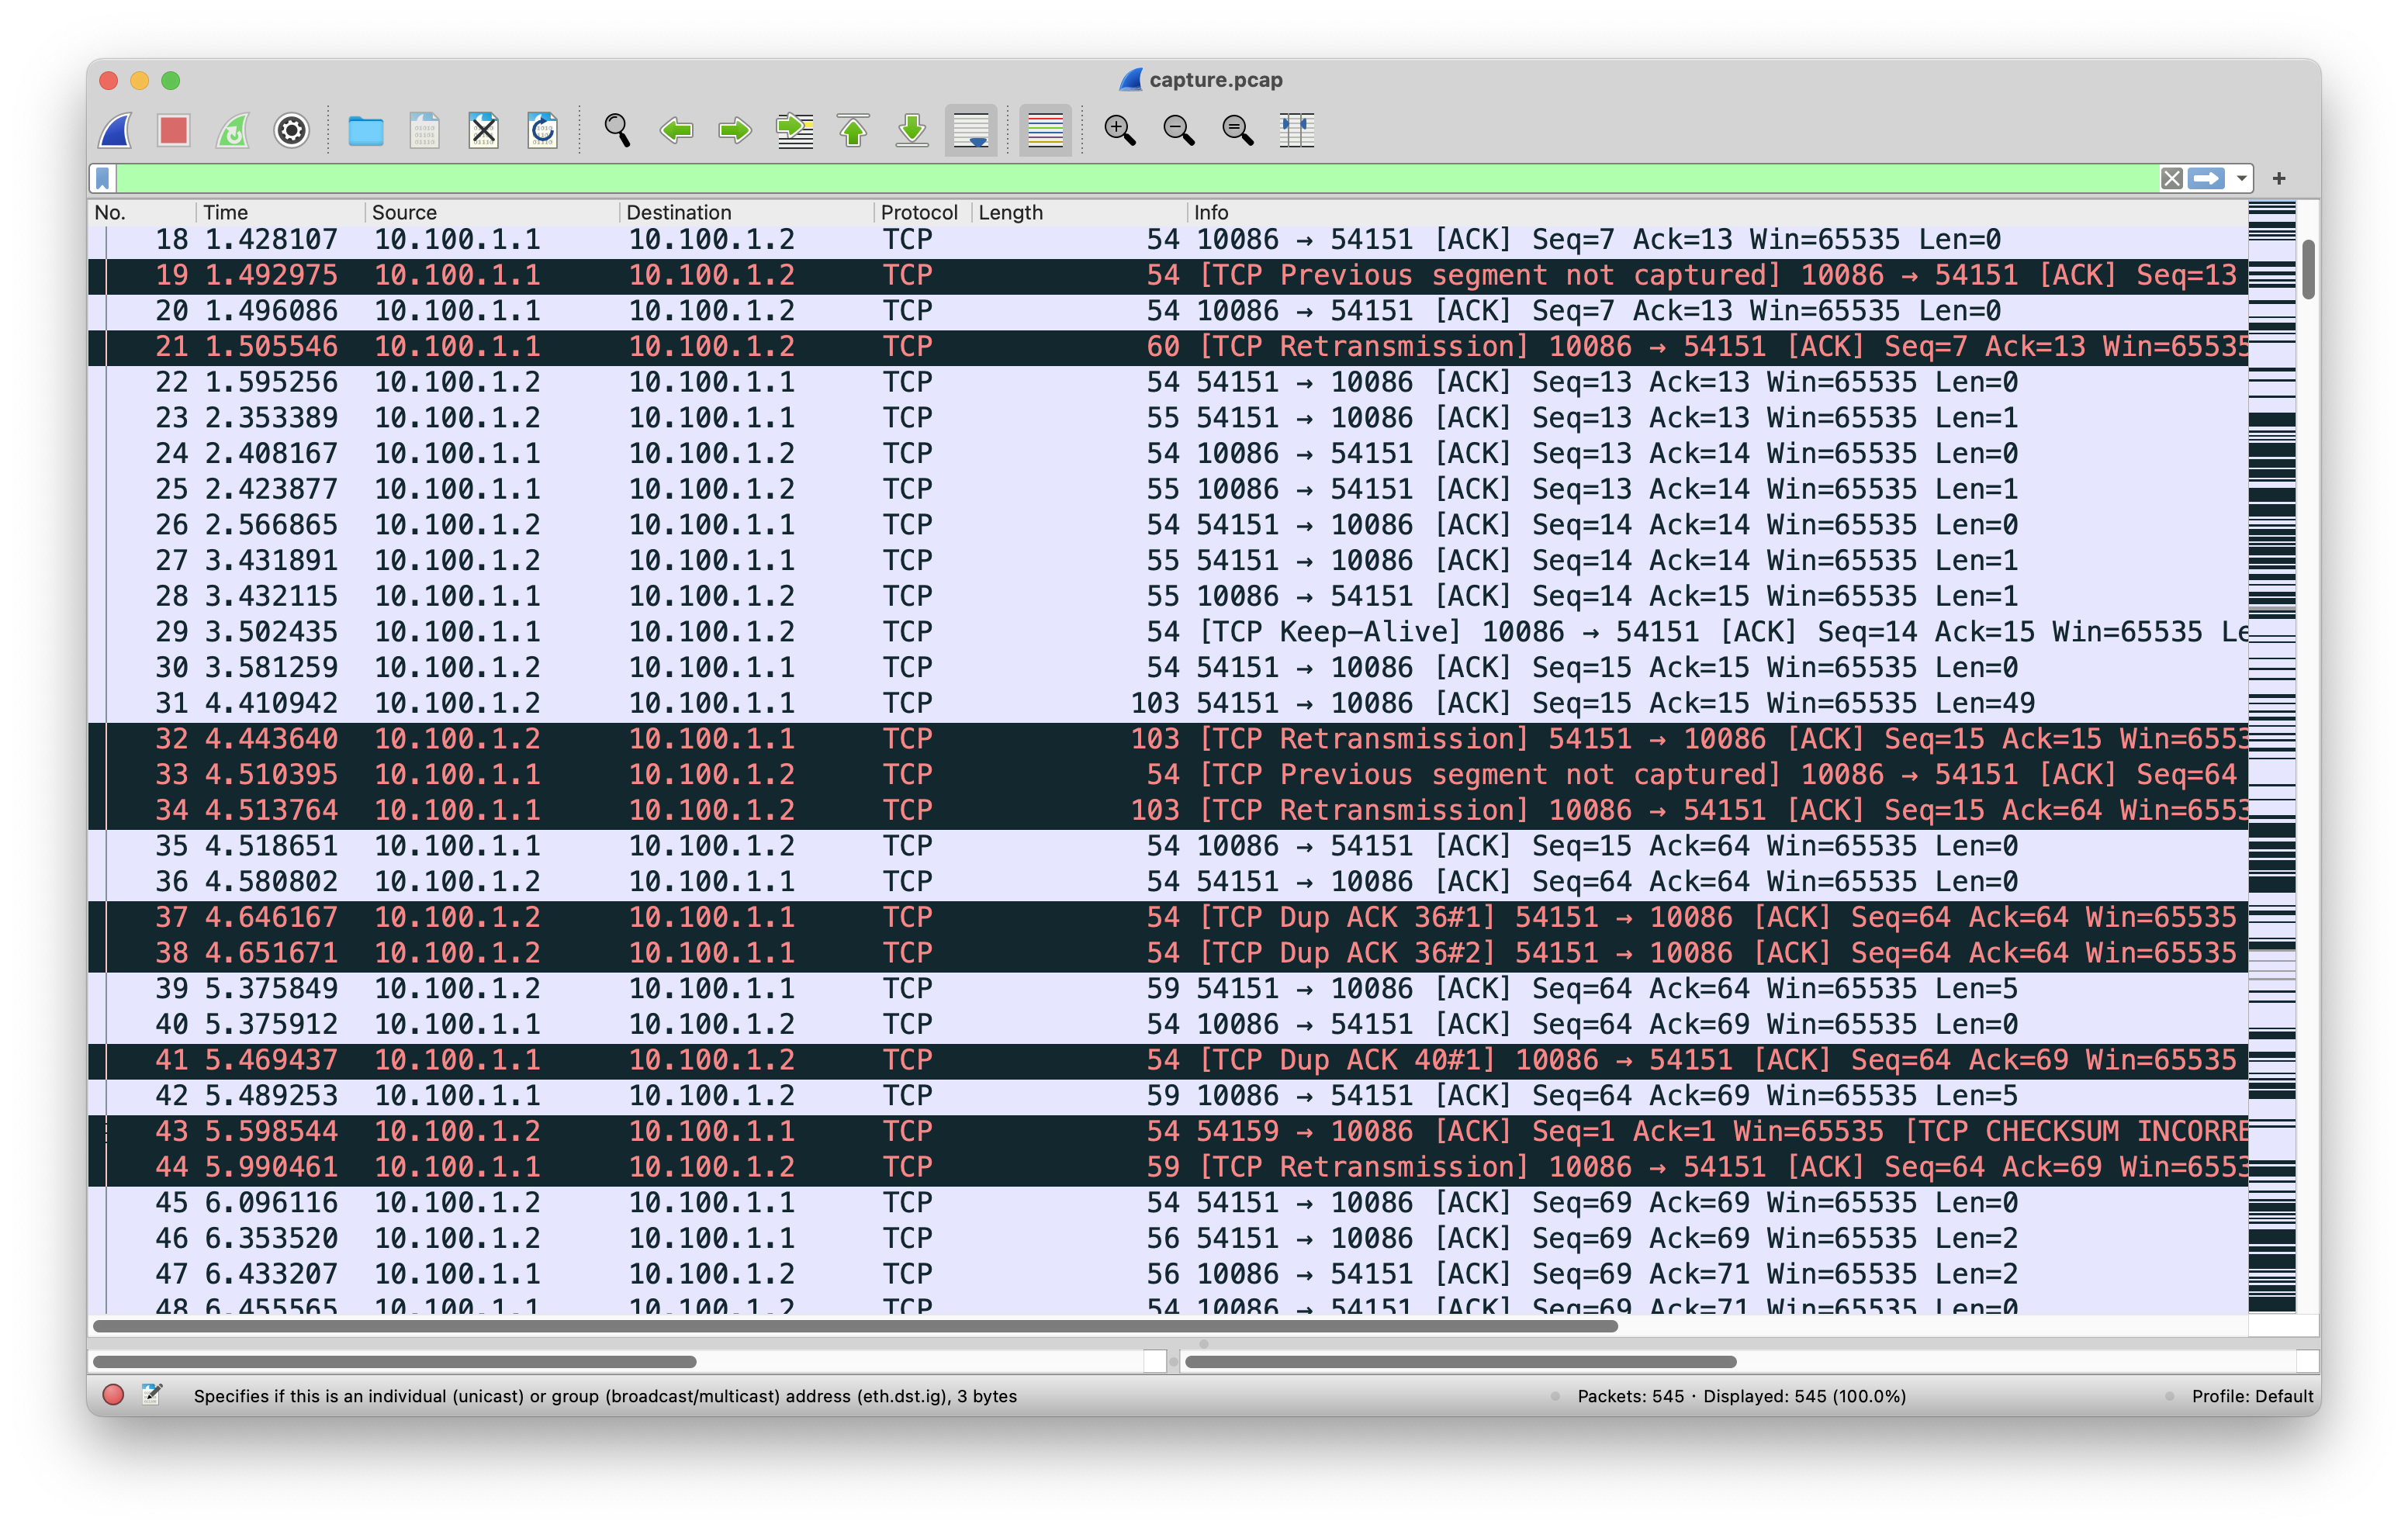
\includegraphics[width=\textwidth]{resources/CP8.png}
    \caption{(Checkpoint 8) Trace of reliable delivery.} \label{fig:CP8}
  \end{figure}

  \subsection{Checkpoint 9 (CP9)}

  The typescript record is at \texttt{checkpoints/CP9/\{typescript, timing.log\}}.

  The output of the application is (the debug output, which exists only in DEBUG build, is removed):
  \begin{minted}{text}
new connection
loop #1 ok.
6 12 13 14 63 68 70 72 74 76 78 80 82 84 86 87 88 89 1113 4184
5208 8279 9303 12374 13398 15000 all: 15000
new connection
6 12 13 14 63 68 70 72 74 76 78 80 82 84 86 87 88 89 4184 8279
12374 15000 all: 15000
loop #2 ok.
new connection
6 12 13 14 63 68 70 72 74 76 78 80 82 84 86 87 88 89 1113 4184
5208 8279 9303 12374 13398 15000 all: 15000
loop #3 ok.
  \end{minted}

  \subsection{Checkpoint 10 (CP10)}

  The typescript record is at \texttt{checkpoints/CP10/\{typescript, timing.log\}}.

  The output of the application is:
  \begin{minted}{text}
sending ...
new connection
receiving ...
1708.82 KB/s
sending ...
receiving ...
1477.72 KB/s
sending ...
receiving ...
1994.34 KB/s
sending ...
receiving ...
2036.69 KB/s
sending ...
receiving ...
1245.22 KB/s
sending ...
receiving ...
3037.36 KB/s
sending ...
receiving ...
1972.81 KB/s
sending ...
receiving ...
2030.82 KB/s
sending ...
receiving ...
2042.39 KB/s
sending ...
receiving ...
2538.34 KB/s
all: 1460000
  \end{minted}

\end{document}
